\section[LodeSTAR Paper]{LodeSTAR: Self-supervised Object Detection}

\begin{frame}[plain]
\begin{center}
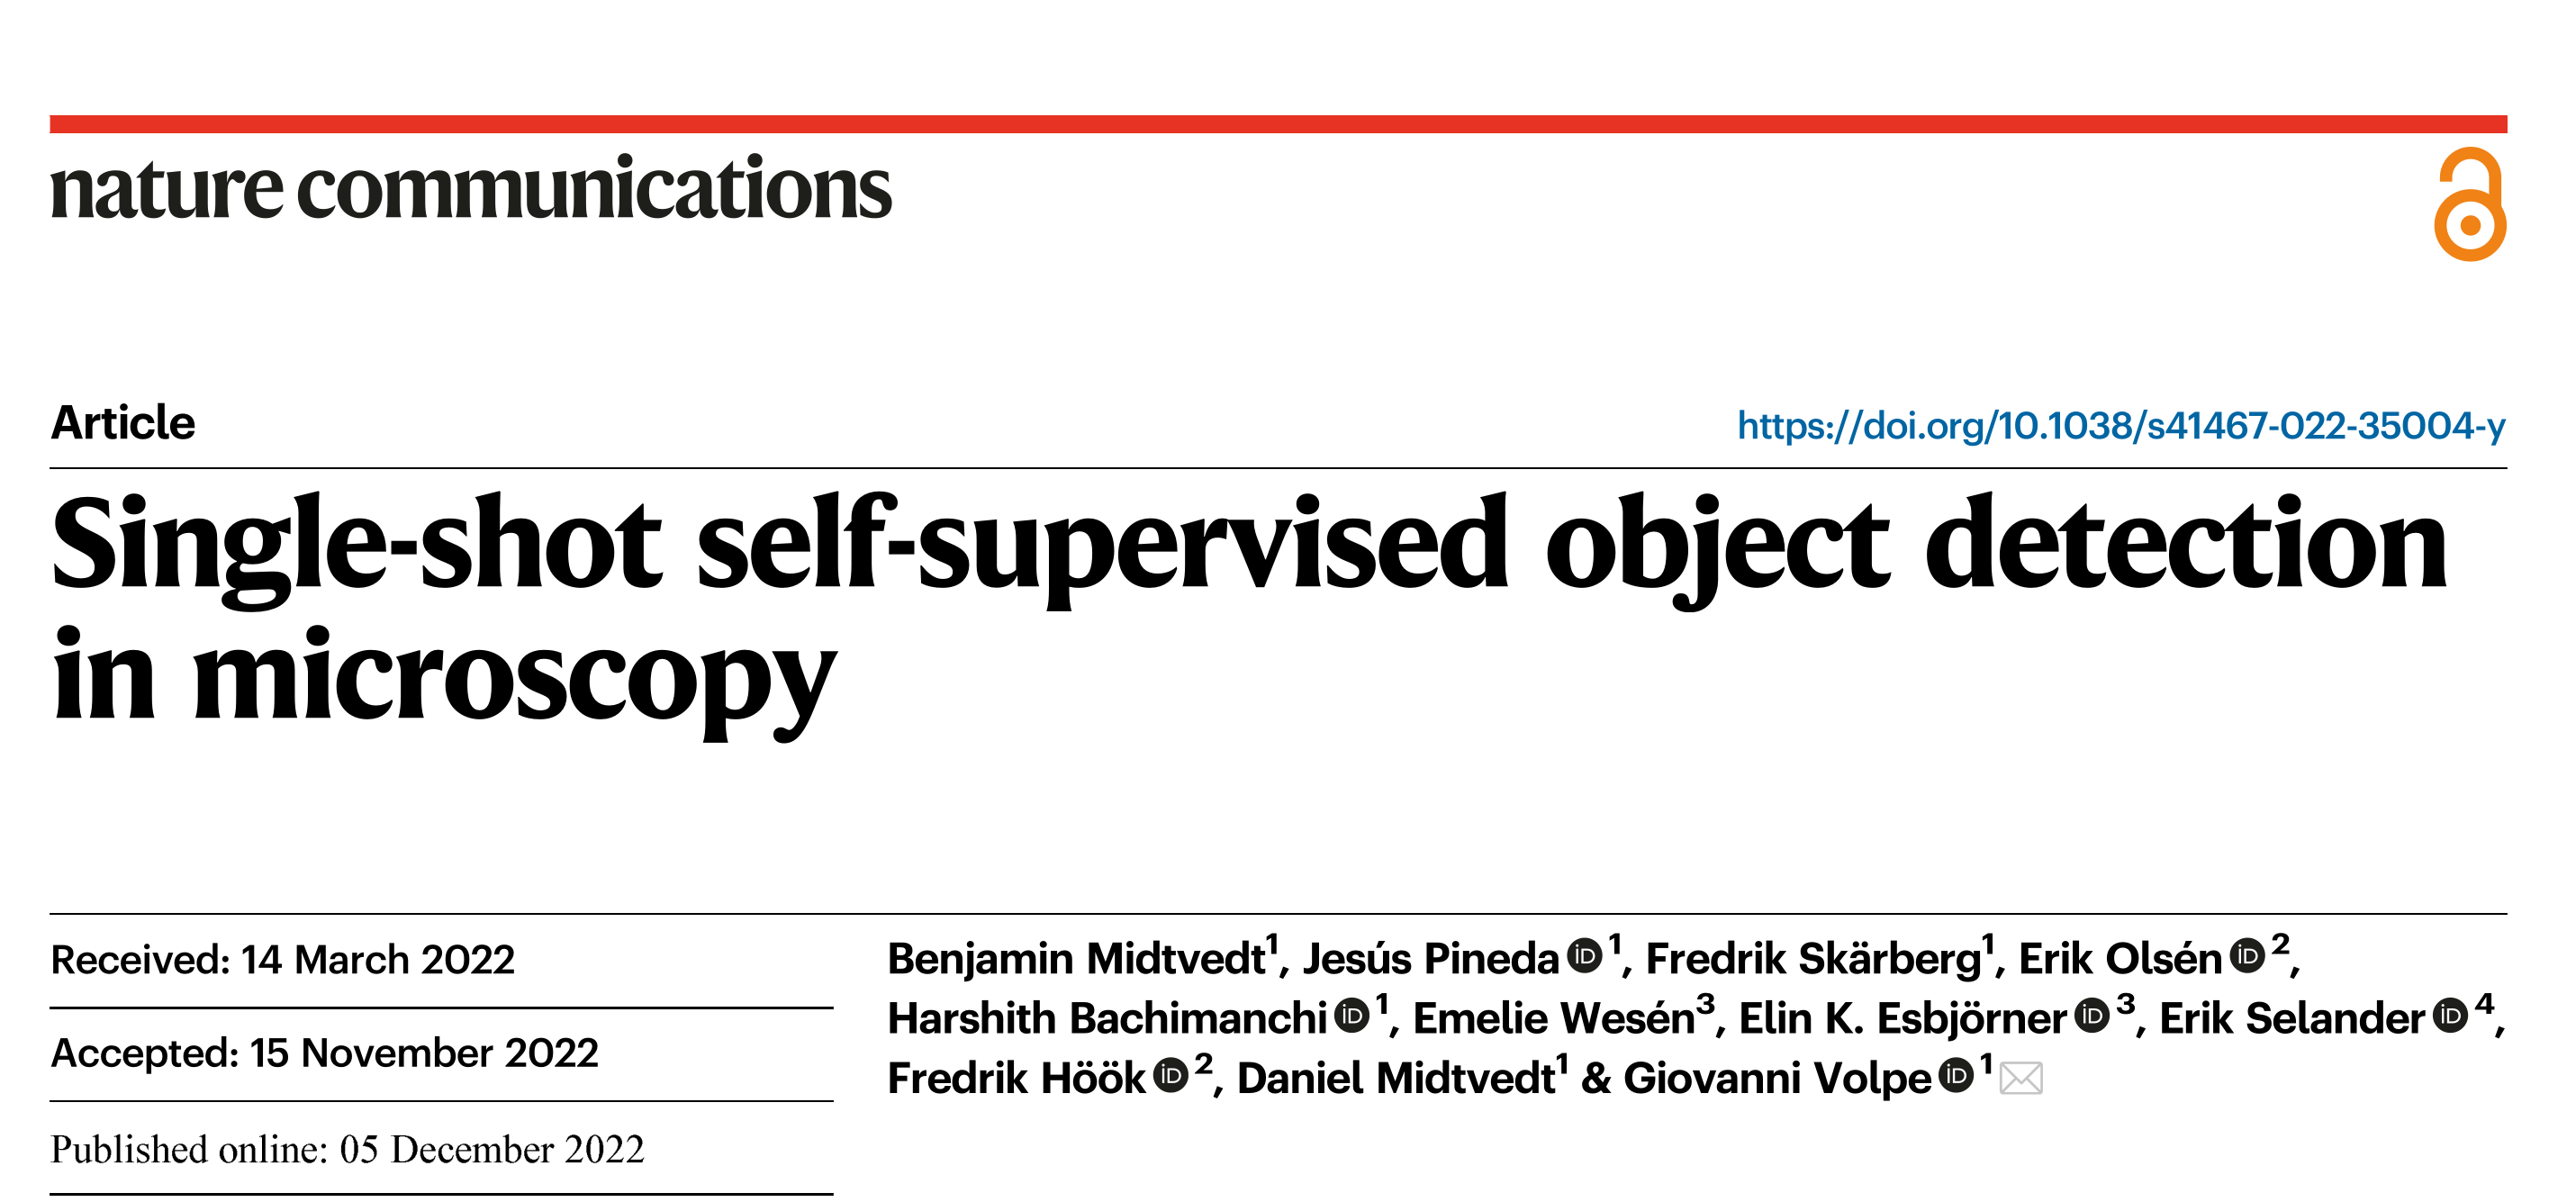
\includegraphics[width=\textwidth]{imglib/Paper_first_page.png}
\end{center}
\end{frame}

\begin{frame}{What is LodeSTAR?}
\begin{itemize}
    \item \textbf{LodeSTAR}: \textbf{Lo}calization and \textbf{de}tection from \textbf{S}ymmetries, \textbf{T}ranslations, And \textbf{R}otations
    \item \textbf{Goal}: Detect objects in microscopy images without manual annotations
    \item \textbf{Key Innovation}: Self-supervised learning using data transformations
    \item \textbf{Output}: Dense predictions of object positions and confidence weights
\end{itemize}
\end{frame}

\begin{frame}{Core Concept: Self-supervised Learning}
\begin{itemize}
    \item \textbf{No manual labels required}
    \item \textbf{Data transformations} create supervision signal
    \item \textbf{Consistency across transformations} = learning objective
    \item \textbf{Translation equivariance} ensures robust detection
    \item \textbf{Process:}
        \begin{itemize}
            \item Transform input image
            \item Train model to predict consistent outputs
            \item Use consistency as supervision signal
        \end{itemize}
\end{itemize}
\end{frame}

\begin{frame}{Geometric self-distillation: Equivariance principle}
\vspace{-0.5cm}
\begin{figure}
    \centering
    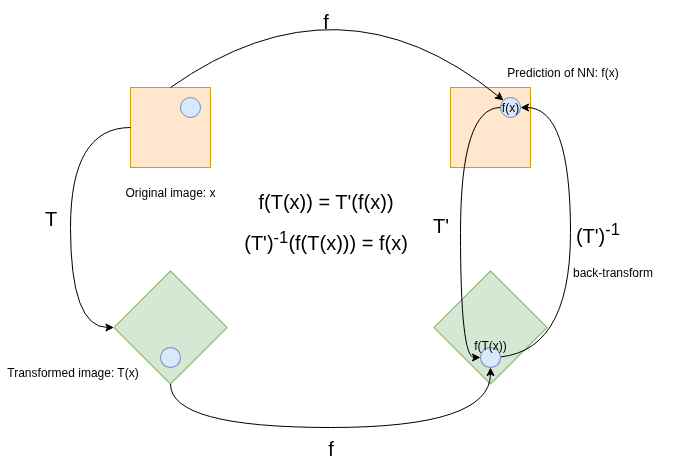
\includegraphics[width=0.6\textwidth]{imglib/maps.png}
\end{figure}
\end{frame}

\begin{frame}{Training}
\begin{figure}
    \centering
    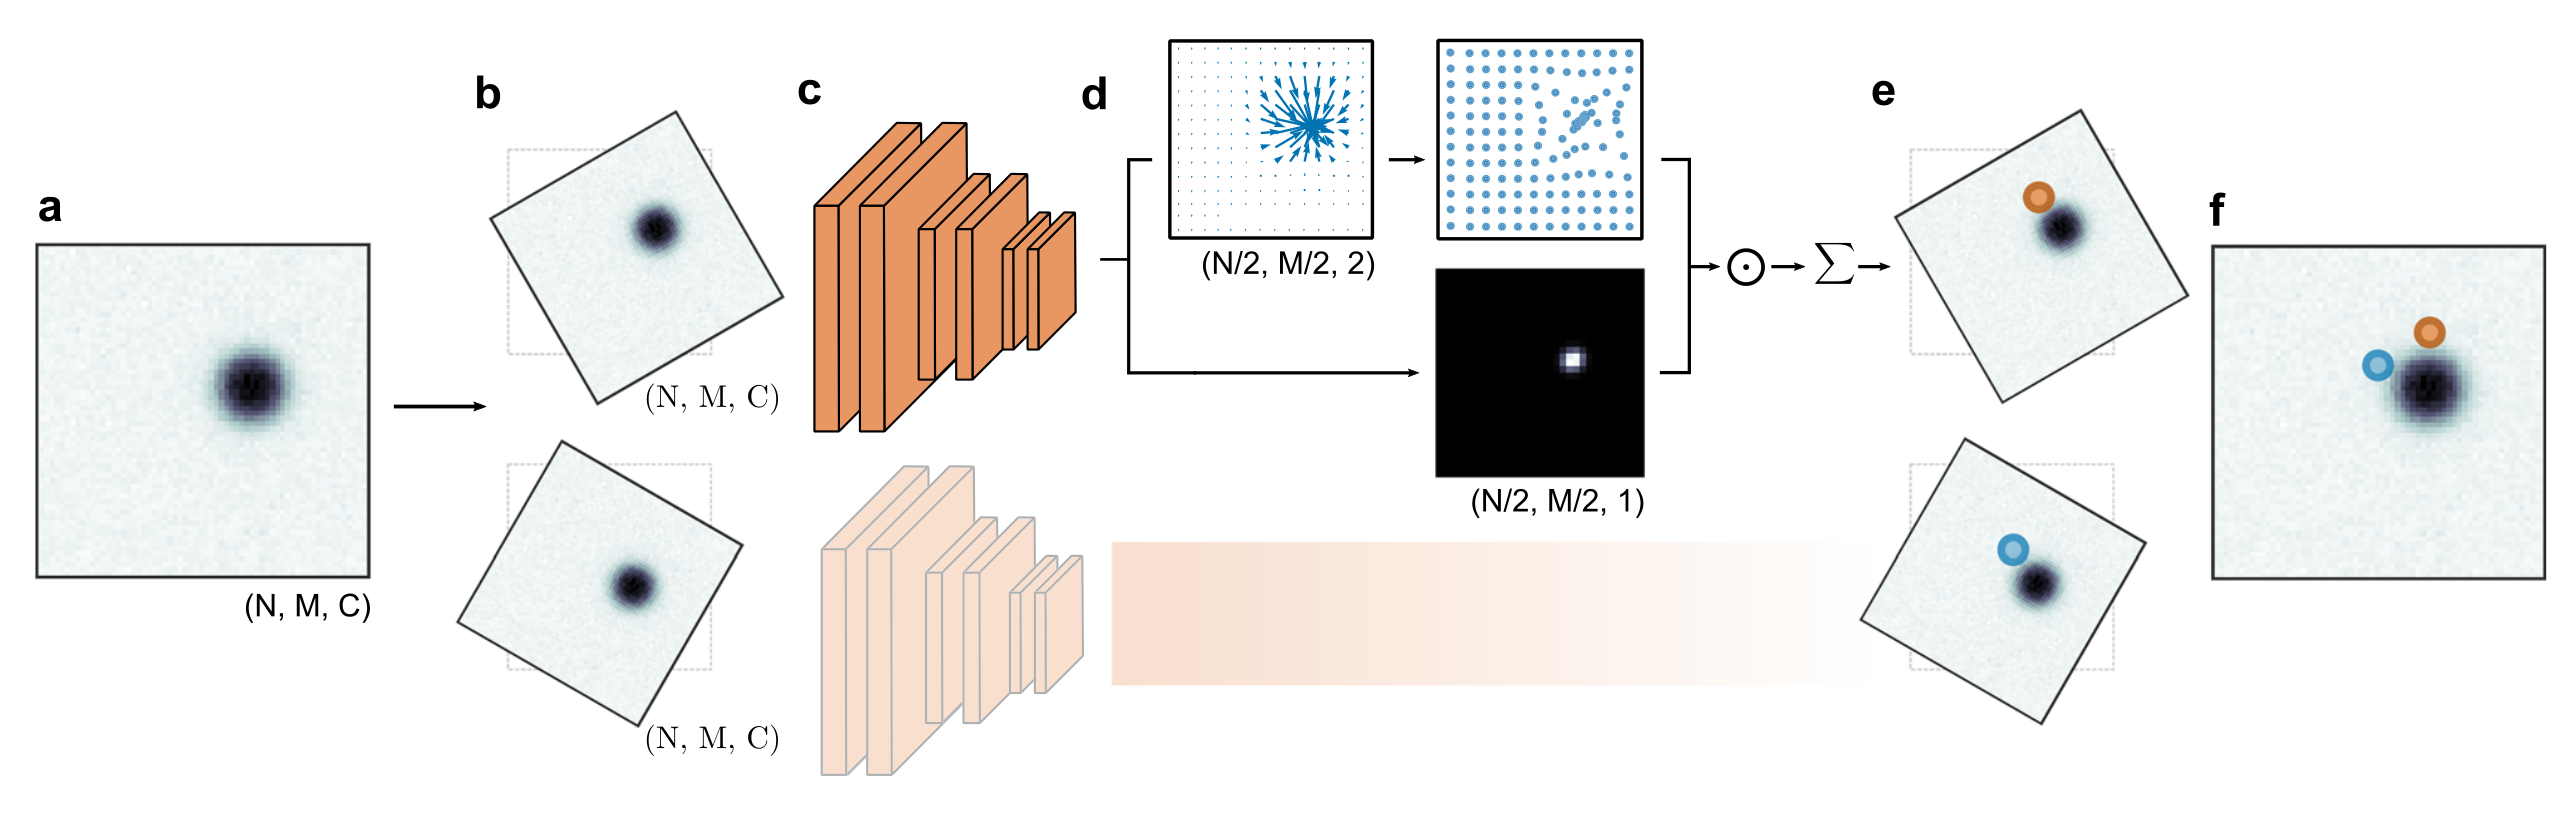
\includegraphics[width=0.8\textwidth]{imglib/single_shot_diagram.png}
    \begin{flushright}
        \footnotesize\cite{Midtvedt2022}
    \end{flushright}
\end{figure}
\vspace{-1cm}
{\small
\begin{itemize}
    \item \textbf{Data Augmentation}: Apply $k$ transformations to input image
    \item \textbf{CNN Processing}: Process transformed images through CNN
    \item \textbf{Parameter Optimization}: Optimize parameters to minimize consistency loss
\end{itemize}
}

\end{frame}

\begin{frame}{LodeSTAR Network Architecture}
\begin{columns}
\begin{column}{0.48\textwidth}
\textbf{Backbone:}
\begin{itemize}
    \item \textbf{Input}: 1-channel grayscale image
    \item \textbf{3$\times$ Conv2D (3$\times$3, 32)} + ReLU
    \item \textbf{MaxPool2D (2$\times$2)} after 3rd layer
    \item \textbf{8$\times$ Conv2D (3$\times$3, 32)} + ReLU
    \item \textbf{Conv2D (1$\times$1, 3)} $\rightarrow$ outputs: $\Delta x$, $\Delta y$, $\rho$
\end{itemize}
\end{column}
\begin{column}{0.52\textwidth}
\textbf{Core Design Features:}
\begin{itemize}
    \item Uniform 32-channel depth
    \item Translation-equivariant
    \item Dense prediction at every pixel
    \item Lightweight: $\sim$100K parameters
    \item No fully connected layers
\end{itemize}
\end{column}
\end{columns}
\end{frame}

\begin{frame}{Architecture Summary Table}
\begin{center}
\begin{tabular}{|c|c|c|c|}
\hline
\textbf{Layer(s)} & \textbf{Type} & \textbf{Channels} & \textbf{Kernel} \\
\hline
0--2 & Conv2D + ReLU & 1$\rightarrow$32 & 3$\times$3 \\
\hline
3 & MaxPool2D & -- & 2$\times$2 \\
\hline
4--11 & Conv2D + ReLU & 32$\rightarrow$32 & 3$\times$3 \\
\hline
12 & Conv2D & 32$\rightarrow$3 & 1$\times$1 \\
\hline
\end{tabular}
\end{center}
\vspace{0.5em}
\textbf{Purpose:} Regress vector field $(\Delta x, \Delta y)$ and confidence $\rho$ from input image with minimal architecture.
\end{frame}

\begin{frame}{Loss Functions}
\vspace{-0.5cm}
\begin{columns}
\begin{column}{0.5\textwidth}
\textbf{Within-image Consistency:}
\begin{align}
L_{\text{within}} &= \| y_{\text{pred}} - \bar{y} \| \cdot w \\
\bar{y} &= \sum w_i y_i / \sum w_i
\end{align}
\begin{itemize}
    \item $L_{\text{within}}$: Enforces agreement between all pixel-wise predictions and the consensus (mean) location
    \item Encourages confident regions to dominate the final prediction
\end{itemize}
\end{column}
\begin{column}{0.5\textwidth}
\textbf{Between-image Equivariance:}
\begin{align}
L_{\text{between}} &= \| y^{T}_{\text{pred}} - T(\bar{y}) \|
\end{align}
\begin{itemize}
    \item $L_{\text{between}}$: Ensures predictions remain consistent under transformations
    \item Encourages the network to learn transformation-equivariant representations
\end{itemize}
\end{column}
\end{columns}
\vspace{1em}
\centering\textbf{Total:} $L_{\text{total}} = L_{\text{within}} + L_{\text{between}}$

\end{frame}

\begin{frame}{Output Processing \& Detection}
\begin{columns}
\begin{column}{0.6\textwidth}
\textbf{Output Components:}
\begin{itemize}
    \item \textbf{Delta X}: X-displacement field (H/2$\times$W/2)
    \item \textbf{Delta Y}: Y-displacement field (H/2$\times$W/2)  
    \item \textbf{Weights}: Confidence scores (H/2$\times$W/2)
    \item \textbf{Sigmoid} applied to weights (0-1 range)
    \item \textbf{Coordinate grids} for absolute positions
\end{itemize}
\end{column}
\begin{column}{0.4\textwidth}
\textbf{Detection Process:}
\begin{enumerate}
    \item \textbf{Forward pass} through trained model
    \item \textbf{Extract} $\delta_x$, $\delta_y$, weights
    \item \textbf{Apply sigmoid} to weights
    \item \textbf{Generate coordinate grids}
    \item \textbf{Calculate absolute positions}
    \item \textbf{Find local maxima} in confidence map
    \item \textbf{Apply threshold} for final detections
\end{enumerate}
\end{column}
\end{columns}
\end{frame}

\begin{frame}{Detection Scoring Metric}
    \textbf{Detection Score Calculation:}
    \begin{itemize}
        \item The model predicts a weight map ($w$) and local consistency ($b$) is calculated from the predictions.
        \item The final detection score ($S$) combines these metrics using geometric weighting:
        \begin{equation*}
            S = w^\alpha \cdot b^\beta
        \end{equation*}
        \item \textbf{Parameters:}
        \begin{itemize}
            \item $\alpha, \beta$: Weights for confidence ($w$) vs consistency ($b$)
            \item \textbf{Cutoff}: Threshold for valid detections
        \end{itemize}
    \end{itemize}
\end{frame}

\begin{frame}{Detection Scoring Metric}
    \begin{itemize}
        \item \textbf{Local Consistency ($b$):} Inverse of local variance of feature maps ($X$) in a $3\times3$ window:
        \begin{equation*}
            b_{ij}^{-1} = \sum_{c=1}^{C} \left[ \left( \sum_{j'=j-1}^{j+1} \sum_{i'=i-1}^{i+1} \frac{{X^c_{i'j'}}^2}{9} \right) - \left( \sum_{j'=j-1}^{j+1} \sum_{i'=i-1}^{i+1} \frac{X^c_{i'j'}}{9} \right)^2 \right]
        \end{equation*}
    \end{itemize}
\end{frame}

\begin{frame}{Summary}
\begin{itemize}
    \item \textbf{Single-Shot}: Detects objects in one pass without region proposals.
    \item \textbf{Self-Supervised}: Learns from geometric symmetries, removing the need for manual annotations.
    \item \textbf{Data Efficient}: Works well with limited training data due to equivariance constraints.
    \item \textbf{Lightweight}: Simple CNN architecture ($\sim$100k parameters) trainable on standard consumer GPUs.
\end{itemize}
\end{frame}